\documentclass[12pt, a4paper]{article}
\usepackage[utf8]{inputenc}
\usepackage{listings}
\usepackage[IL2]{fontenc}
\usepackage[czech]{babel}
\usepackage{graphicx}
\usepackage{mathtools}
\usepackage{amsmath}
\usepackage[pdfborder={0 0 0}]{hyperref}

\title{\textbf{Dokumentace semestrální práce} \\KIV/MBKZ}
\author{Vojtěch Danišík}
\begin{document}

\begin{titlepage} 
	\newcommand{\HRule}{\rule{\linewidth}{0.5mm}} 
	\begin{center}
	
\includegraphics[width=6cm]{img/logo}\\
	\end{center}
	\textsc{\LARGE Západočeská univerzita v~Plzni}\\[1.5cm] 	
	\textsc{\Large Mobilní komunikace a zařízení}\\[0.5cm] 
	\textsc{\large KIV/MBKZ}\\[0.5cm] 
	\HRule\\[0.4cm]
	{\huge\bfseries Dokumentace semestrální práce}\\[0.4cm] 
	\HRule\\[1.5cm]

	\begin{minipage}{0.4\textwidth}
		\begin{flushleft}
			\large
			Vojtěch \textsc{Danišík}\newline
			A19N0028P\newline
			danisik@students.zcu.cz
		\end{flushleft}
	\end{minipage}
	\vfill\vfill\vfill
	\begin{flushright}
	{\large\today}
	\end{flushright}
	\vfill 
\end{titlepage}
\newpage
\tableofcontents
\newpage
\section{Zadání}
Jako zadání semestrální práce pro předmět MBKZ byla vybrána hra \textbf{Piškvorky - TicTacToe}. Hlavní podstatou piškvorek je sestavit řadu o velikosti 5 po sobě jdoucích značek. Značky můžou být v diagonálních směrech, zleva doprava a odshora dolů. Hra se hraje ve dvou, kdy první hráč má značku \textbf{X} a druhý hráč má značku \textbf{O}. Za hráče se může považovat člověk i počítač. Hráči se snaží dosáhnout vítězné řady ale zároveň zabránit seskládání vítězné řady u protihráče. Vzhled této hry lze vidět na obrázku \ref{fig:uvod_obrazek}.
	\begin{figure}[h!]
	\centering
	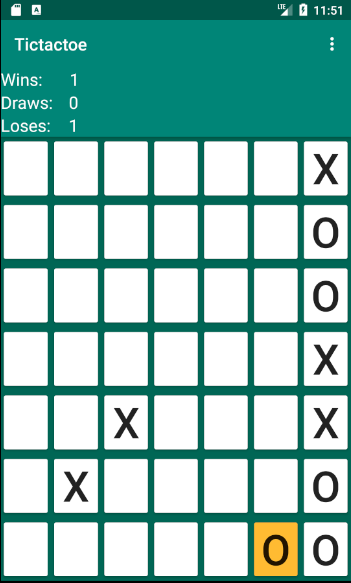
\includegraphics[width=5cm]{img/highlighted}\\
	\caption{Piškvorky - ukázka}
	\label{fig:uvod_obrazek}
	\end{figure}
\newpage


\section{Programátorská dokumentace}
%TODO
V~programu bylo použito pro docílení správné funkcionality 7 tříd.
\par
Třída \textbf{MainActivity} slouží jako hlavní třída aplikace. V~této třídě se děje zobrazování již vytvořených struktur jako jsou například vytváření tlačítek, hracího pole, přiřazování aktivit tlačítkům.
\par
Třída \textbf{PlayerEngine} slouží pro zjištění tahu pro počítač. Pro zjištění tohoto tahu byl implementován algoritmus \textbf{Depth-First Search} algoritmus, který je ale omezen na maximální hloubku 4.
\par
Třída \textbf{Constants} obsahuje veškeré konstanty použité v aplikaci.
\par
Třída \textbf{Node} slouží jako jednoduchá reprezentace tlačítek při zjišťování tahu pro počítač.
\par
Třída \textbf{CustomButton} je rozšířením základního tlačítka v android studiu. Obsahuje dodatečné informace při práci s hledáním v poli - souřadnice X a Y a také který hráč označil dané tlačítko.
\par
Třída \textbf{MainActivity} slouží jako hlavní třída aplikace. V~této třídě se děje zobrazování již vytvořených struktur, jako jsou například časovač, hrací panel ale také i přiřazování aktivit pro tlačítka RESET a SET FLAG.
\par
Třída \textbf{EGameStatus} je enum, která reprezentuje aktuální stav hry.
\par
Třída \textbf{MoveChecker} slouží k zjištění, zda aktuální tah vedl k výhře hráče. 
\newpage


\section{Uživatelská dokumentace}
Výsledný vzhled aplikace lze vidět na několika obrázcích. První obrázek (viz \ref{fig:title}) vyobrazuje aplikaci po jejím spuštění, kdy si hráč vybírá velikost mapy z tří zvolených možností (5x5, 6x6, 7x7). Aplikace navíc obsahuje počítadla výher/remíz/proher prvního hráče (Vás).
	\begin{figure}[h!]
	\centering
	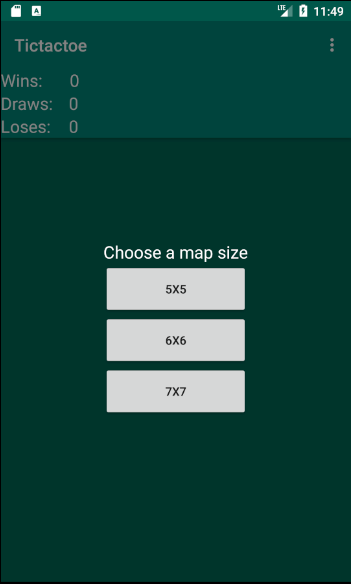
\includegraphics[width=5cm]{img/title}\\
	\caption{Vybrání velikosti hracího pole}
	\label{fig:title}
	\end{figure}
\par
Po výběru velikosti mapy aplikace vygeneruje hrací pole o zvolené velikosti a čeká, než první hráč (vy) zahájí hru prvním tahem. Příklad vygenerované mapy 7x7 lze vidět na obrázku \ref{fig:board}.
\newpage
	\begin{figure}[h!]
	\centering
	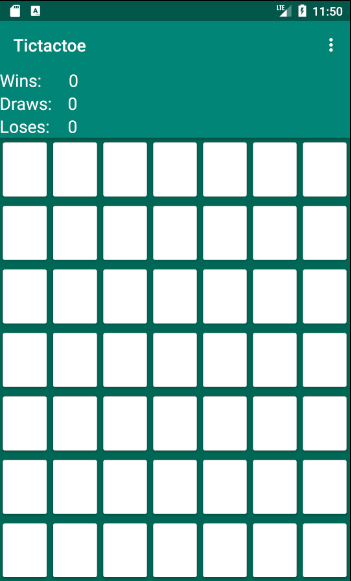
\includegraphics[width=5cm]{img/board}\\
	\caption{Vygenerované hrací pole}
	\label{fig:board}
	\end{figure}
\par
Jakmile uživatel klikne na jakékoliv pole na hrací ploše, označí se toto pole značkou \textbf{X} a už na něj nelze kliknout. Po odehrání hráčovo tahu bude hrát počítač, který podle implementovaného algoritmu vybere nějaké políčko a to označí značkou \textbf{O} Políčko zvolené počítačem bude zároveň označené žlutou barvou, aby mohl první hráč zjistit, které políčko vybral počítač. Příklad vybraného políčka počítačem lze vidět na obrázku \ref{fig:move}.
	\begin{figure}[h!]
	\centering
	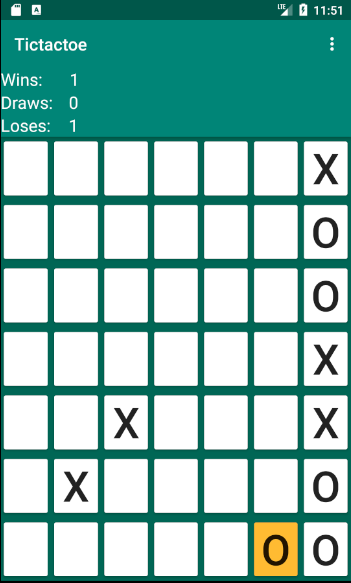
\includegraphics[width=5cm]{img/highlighted}\\
	\caption{Tah počítače}
	\label{fig:move}
	\end{figure}
\newpage
Hra končí, pokud jeden z hráčů poskládá vítěznou kombinaci (o velikosti 5) a nebo všechny políčka budou zabraná, aniž bude existovat vítězná řada, tudíž vznikne remíza. Po dohrání hry jsou aktualizovány statistiky a uživatel může začít novou hru zvolením nové velikosti hracího pole. Příklad dohrání hry do úplného konce lze vidět na obrázku \ref{fig:endgame}.
	\begin{figure}[h!]
	\centering
	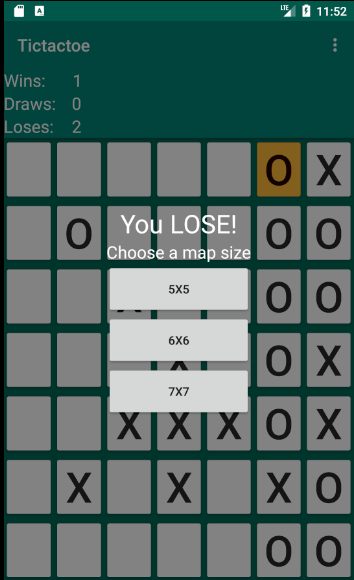
\includegraphics[width=5cm]{img/endgame}\\
	\caption{Konec hry}
	\label{fig:endgame}
	\end{figure}
\newpage


\section{Řešené problémy}
Při vyvíjení aplikace jsem narazil na jeden jediný problém, a to byla časová náročnost řešících algoritmů pro AI. Jako první jsem měl naimplementován algoritmus \textbf{Minimax} a jeho rozšíření \textbf{Alpha-beta prunning}, bohužel pro hrací pole větší jak 3x3 byla časová doba pro jeden tah AI velice dlouhá a nepodařilo se mi implementovat limitaci algoritmu podle hloubky zanoření. Následně jsem použil nejjednodušší řešení, a to algoritmus \textbf{Depth-First Search}. Pro tento algoritmus byla taktéž časová doba pro tah AI víceméně stejná jako u předchozích algoritmů ale s tím rozdílem, že se mi podařilo implementoval limitaci podle hloubky zanoření. Maximální zanoření DFS může být maximálně 4 a to z důvodu přijatelné hrací doby jednoho tahu AI pro hrací pole 7x7.
\newpage


\section{Testování}
Aplikace byla vyvíjena a testována v~Android Studiu verze 3.5.3 (od firmy JetBrains) v~jazyce JAVA. Při vývoji bylo využito JRE verze 1.8.0\_202. Jako testovací mobil byl vybrán Pixel 2 s~API verzí 24 a operačním systémem Android ve verzi 7.0 (Nougat). 
\newpage


\section{Závěr}
Vytvořená mobilní aplikace \textbf{TicTacToe}, neboli piškvorky, splňuje základní funkcionalitu stejnojmenné hry. Uživatel je schopný hru bezproblémově dohrát a ukončit ji v~jakémkoliv případě. Ovládání aplikace je velice jednoduché, stačí pouze klikat na políčka v~hracím poli a podle zobrazeného čísla u~některých políček odhadovat, na jakém políčku se můžou nacházet bomby. Bomby jsou rozmístěny náhodně, v~každé hře jsou na jiné pozici. 
\par
Při testování se nevyskytly žádné chyby, které by měli zásadní vliv na funkčnost aplikace. Testovány byly především všechny stavy, které se mohli u~této hry vyskytnout, jako například výhra/remíza/prohra nebo třeba kliknutí již vybraného políčka.

\end{document}